% -*-latex-*-
% Typical article template

\documentclass[a4paper,10pt]{article}
\usepackage{amsmath}
\usepackage{amstext}
\usepackage{amsbsy}
\usepackage{graphicx}
\title{ MEDIC Extends DICOM Imaging and Communications \\
\textit{Design and Architecture} }

\author{Eray {\"O}zkural}

\date{\today}

\begin{document}

\maketitle
\begin{abstract}
DICOM standard is a main concern in the development
because of its prominence in medical imaging. At the RAGARIS project,
many alternatives have been considered in early design and it has been
decided that an in house library implementation suits the needs of the project
better.
The design and implementation has undergone a long period of development and the
software is in operational state.
This document describes various design issues and technical details of the
MEDIC software that makes digital medicine applications DICOM compliant.
\end{abstract}

\section{Introduction}

Through many years of worldwide experience of digital medicine, a standard
known as DICOM has emerged. The standard is a thorough collection of
documents which determine many aspects of operation and communication of
devices which support digital imaging in medicine. It has been the de facto
industry standard for years and the most recent one is DICOM 3.0 that was
published by NEMA in 1997.

In brief, the standard directly addresses the communication, storage and
retrieval of medical imaging data, and other aspects of digital systems such
as a patient information system and printing. It is not the purpose of this
report to duplicate the numerous definitions and protocols of the DICOM
standard in this document. Rather, the reader is encouraged to refer to the
standard itself. Though lengthy, many of the main issues are to be best
found in the 14 parts of the standard. The emphasis of this document is on
our design and implementation of DICOM 3.0.

The standard is based on an object oriented information model to be able to
account for the conceptual depth and flexibility required by a medical
imaging system. The message passing (over TCP/IP), distributed, persistent
object system makes realization of a versatile and sizable PACS possible.
Once dealt appropriately DICOM makes things easier. However, DICOM itself is
fairly big: the current implementation supports the 24*5 primitive data
types (see PS3.5), 895 attribute types (see PS3.6), 103 information module
classes, 35 information object classes (composite and normalized, see PS3.3)
and 25 messages (see PS3.7). Obviously, DICOM represents many technical
challenges caused by its sheer complexity. Clear design directions had to be
taken, and most features of the standard have been successfully implemented.

This report describes the library by first
%giving a summary of system
%functionality, then
elucidating the design issues. Consequently, we 
report an overview of architectural components and supply a class
reference at a medium level of detail which furnishes insight into the
implementation.

\section{System Overview}

MEDIC is a library that aims to be a complete and conformant
implementation of the DICOM 3.0 standard. It is assumed throughout
the document that the reader is familiar with the standard and its medical
applications; no further attempt will be made to explain the issues within
the scope of the standard. Since the standard explicates protocols and
behavior, leaving the implementation details unspecified, there is a host
of choices for the implementor to make. In particular, one chooses
which subset of the standard he shall aim to implement, which platform
the implementation is going to work on thus how application software
will use it for DICOM compliance.

MEDIC achieves this by a faithful translation of the standard to
a library that is a collection of programming interfaces which
are invoked by DICOM applications. It has been meant to be a portable,
comprehensible, reliable, efficient, extensible and rigorous implementation.

It is a framework under which application programmers write DICOM
code conveniently. When an application works with MEDIC, 
it behaves as a DICOM Application Entity  which can interoperate
with other Application Entities. Basically, it allows the programmer
to manage DICOM objects \footnote{construct, destruct, select/modify
attributes, pass pointers to them}, and apply various
DICOM operations including operations over TCP/IP and media storage.
The design exclusively tries to hide implementation details from the
user, and gives him abstract services. That's where MEDIC extends
DICOM. For instance, any application entity started automatically
becomes SCP for most service classes as well as SCU. Many difficult
aspects of the implementation are not presented to the user, for
instance all association happens automatically and user sends commands
over an association with simple constructs.

In summary, MEDIC implements majority of the standard, excluding
most notably OSI upper layer services and legacy 50-pin connection
which are both obsolete.

\section{Design Considerations}

\subsection{Background}

A major standard is usually prepared in terms of existing systems and
standards. DICOM is no exception; it leans on concepts from object-oriented
systems (IOD, services), databases (E-R diagrams), networked environments
(Application Entity, Association, Transfer Syntax); also it incorporates
many international standards by ISO, ANSI and IEEE. Nevertheless, the
standard introduces several proprietary terms and concepts which are
specific to DICOM, and in many cases, it is hard to tell which design would
be better since the standard avoids giving such an advice.

Therefore, the implementations led by development teams elsewhere have
followed quite different designs. For instance, an implementation works with
run-time classes, and interesting functions to manipulate objects of those
classes and send/receive messages. Another implementation keeps attribute
types in a database, and queries the database for type checking. These may
look clumsy, but if you need to know just one value from an object, you can
perhaps parse it with a simple code (so that it would skip all irrelevant
data) and fetch what you need. In particular, it is relatively easy to
implement a very small portion of the standard; but whenever one attempts at
a general solution, many hazards appear.

\subsection{Assumptions}

The implementation platform is already set as Windows NT / Microsoft Visual
C++, so our software has to respect the selection. As an object oriented
language, C++ is a suitable candidate for a DICOM implementation. Our
software, named MEDIC, is designed to be close to
ANSI C++, bearing as little dependency on VC++ as possible.

At any rate, MEDIC has been designed to be highly portable and thus
we assume no hardware platform. We anticipate that the library can
be made to run on top of any POSIX or WIN32 API which encompasses
a wide range of hardware from embedded applications to workstations.

The library audience is medical application programmers who require
DICOM compliance in their software. The library is nicely packaged
for both GNU toolchain and Visual C++ so that programmers can quickly
browse the source code and tutorial examples and integrate
MEDIC functionality in their applications rapidly.

Since DICOM is continously evolving, we may expect to account for
corrections and supplements to the standard. In the natural course,
all final versions of the standard and essential drafts will be supported.

\subsection{Constraints}

The library presupposes a rather modest hardware/software setup. We
assume no more than baseline development tools and standard
libraries. In the platform independent portion, we use only ANSI C++
and its standard library. On GNU platforms, the GNU toolchain and
standard socket and thread libraries are utilized. The Visual C++
version uses MFC for all functionality.

The framework is compiled as either a static or shared library
according to the platform. On Visual C++, due to compiler and linker
peculiarities we have to build a static library. The framework
has a simple invocation consisting of only a single initalization
entry point.

The resources used by MEDIC are quite standard, we make use of
file, TCP/IP, multithreading and timer services from underlying OS
through appropriate APIs.

The library is a fairly complete implementation of DICOM and it
implements 11 of the 13 volumes of DICOM 3.0 standard. Since it
uses TCP sockets, the reader is referred to RFC's
detailing TCP/IP protocol.

Interoperability is achieved through DICOM communications over TCP/IP.
MEDIC implements only synchronous mode transfers because there does not
seem to be a good framework for writing convenient asynchronous code
in C++.

Each Application Entity is supposed to run on a single machine. A
DICOM Application Entity has a persistent store of DICOM objects
and distribution is achieved through DICOM store, get and move
commands.

No security measures are taken as we simply assume that anyone
who can make a TCP connection is a trusted party and the system
is open in the sense that it has been designed as an Internet
application protocol. Security against malicious attacks can
be arranged simply by putting critical services inside a private
IP network that is not visible to outside world and placing
public access services on a node that is visible to whole Internet.

The implementation has no hard limits in the tradition of
modern system software. There are however user settings
that may be mentioned here. First, the implementation requires
free secondary storage to store persistent objects. The maximum
memory and disk space used by persistent store is also set by the
user. User can also set the maximum number of open connections
to DICOM server.

Since the application runs in a single user process space, 
message passing overhead is very low. Furthermore, 
binary encoding/decoding is performed on the fly enhancing
performance. The only bottleneck we have observed is
the stdio and iostream implementation on WIN32 platforms.

The applications that use the library have been tested using
Agfa DICOM Validation Tool and DICOMTK. Also, the library has
been stress tested during the development and testing of
RAGARIS PACS applications.

\subsection{Objectives}

Indeed, a DICOM implementation is about realizing an object system
with the characteristics previously mentioned. The main goal of
a DICOM implementation is interoperability. Nevertheless,
interoperability has a cost. Internal representations will have to
be converted to interchangeable representations, the application
will have to implement complex protocols in order to communicate
with other DICOM applications, and behave accordingly to the standard.
For instance, images will be converted from platform specific display
memory to a complicated DICOM object which encapsulates many
attributes about an image having a binary representation
specified in the standard, and vica versa.
Likewise for non-image information such
as study data or reports. This entails in itself providing mandatory
attributes, and a host of binary parsing and generation code at
various levels \footnote{from VR representation to a complete
  Dataset}. The object representations maintained this way are
useless without specifying an operation on them. Typically, one
stores, fetches and manipulates this data on a distributed system
connected with TCP/IP or stores them on storage media such as CD-R.
In doing that each target has its own protocols. Processing over
the network requires conforming to an OO RPC protocol which is the
focus of DICOM3.0. Most services are defined this way, and besides
requiring a plentitude of message passing semantics and a large
protocol FSM, each one has its own service semantics. For instance,
when another application stores an image object on us we should store
it in a persistent way which may be accessed later. Writing and
reading storage media requires directory and file services which also
demand the same attention. Basically the interoperability cost is
incurred by the code that maps application semantics to DICOM
semantics. A DICOM object has many essential features. For instance,
it needs to have a class and instance UID. Having to specify these
special features and communication/storage code is arduous in
traditional implementations. The development cost is further increased
by diminished reliability and poor maintainability of bloated code.

MEDIC aims to cut down this cost by enhancing DICOM development with
an advanced application framework. There are recurrent themes
throughout the implementation. First, each used feature of the
standard is translated into a first class construct in the host
language. That is, we deliberately avoid having anything remotely
similar to various \textit{ad hoc} object models that are constantly
being promoted recently. If there is a class, it is a class in the
language. If there is a type, the implementation is a type in the
language. We stick to exact translation, semantics already present
in the implementation language are used and not augmented with
auxiliary and inferior systems. The second theme is minimizing user
code length. Whatever DICOM task the user wishes to perform, he should
be able to accomplish it with a very short amount of \textit{abstract}
code. In the user codes, we give attention to optimizing the common
cases and still giving a high level of freedom to the programmer.

This being said, we should clarify the design goals mentioned. MEDIC
has the following design goals. In the following text, we describe
in what way the design goal is required and how we have achieved it.
\begin{description}
\item[portable] DICOM applications may be implemented on a wide range
of hardware. Dependence on a particular architecture and operating
system would not be desirable. Although most of the development has
been done on Windows, we have taken care of portability by minimizing
and isolating Windows specific code. The platform independent part
is totally standard C++ and compiles with no difficulty on many
platforms already.
\item[comprehensible] The biggest disadvantage of DICOM is its
size. With so many concepts and symbols to keep track of, programmer
soon gets drowned in the non application specific parts of coding.
We obtain ease of use by taking advantage of object oriented
programming. The interface classes are highly abstract and every
feature in the standard is readily accessible. For instance, changing
an attribute in an IOD is accomplished by a single line
of code which is a usual C++ method call. Sending an image over
network is another one-liner.
\item[efficient] Whenever there are advanced functionality such as
 message passing and persistence, it is possible
to implement it very slowly. In a medical imaging application,
efficiency is cruicial because we have to deal with very large
volumes of data at a high rate.
The library has well tuned code that does
not have any significant overhead which arises from the amount of
abstraction. We use generic programming internally to capture
code similarity rather than less efficient object oriented programming
techniques where necessary. The efficiency however comes not
from avoiding advanced C++ features as they are used where they have
been useful. It comes from the fact that we do not resort to an
artificial type or object system that is not under compiler control
and optimization. When we decode an object, all that is done is
executing plain C++ code on the fly which gives us equivalent
performance to any hand written DICOM parsing routine. Another example
is the way we treat DICOM data types, one can create a VR on stack
or heap, as he wishes; similarly for coarse grained data types such
as modules or IODs.
\item[extensible] Since this is an evolving standard, the
  implementation must be extensible in almost every aspect. In the
current implementation, it is quite easy to add new DICOM classes,
transfer syntaxes and services simply by plugging in required classes
into the code.
\item[rigorous] Most DICOM implementations suffer from incompleteness.
 This is not the case with MEDIC because we employ a compiler that
 generates dataset coder/decoders and an object oriented decomposition
 has been used to enforce mandatory behavior while still allowing
 optional behavior. As a result, we have not yet found many DICOM
 dataset or command that have not been successfully processed by
 our implementation nor has many of generated datasets or commands
 have been interpreted as erroneous by other implementations. We have
 of course spotted bugs in the development which we have fixed and the
current state of the library is quite rigorous in that respect. All
protocol violations depicted in the standard are explicitly checked
and reported if encountered. Thus, for instance it is impossible to
process a faulty dataset: we do not do any sort of fuzzy parsing, but
it is also impossible to send an incomplete object over the network.
\item[reliable] In most other implementations, we see that the
object model is implemented external to the host language and a lot
of awkward function calls are required to do even the most basic
operations. That is not the case with MEDIC, because almost every
operation is through first class constructs which means that strong
type checking, and other reliability features of C++ are fully employed.
\end{description}

\section{Architectural Strategies}

We have used standard system software for developing the library. Most
of the library is standard C++. For the compiler we have used GNU
flex/bison. On windows, MFC is used for platform specific
functionality.

The library has simple exception based error handling. All system
errors and protocol violations are interpreted as exceptions. No
attempt is made to recover from parsing because all DICOM data has to
be well formed.

Memory management and persistence is achieved through a custom virtual
memory system and smart pointers with hooks to the virtual memory. It
consists of LRU paging of objects to disk and modified objects
streamed back to disk occasionally. Persistent objects are scanned at
the beginning of each invocation. User can create either transient or
persistent DICOM objects.

DICOM SCPs are implemented as a multithreaded server. Each service
request is performed concurrently on its own thread and they share
resources such as the persistent object store.

\subsection{Application Framework}

MEDIC is an application framework which provides all the back-end
code for writing DICOM applications. A framework lets the programmer
employ useful abstractions which solve problems in the application
domain and sometimes extend them.

When MEDIC starts up, it configures itself, initialized subsystems
such persistence, spawns a multithreaded server that listens on
the DICOM port, and so on. Much of its functionality is autonomouse,
the application becomes a DICOM AE simply by using MEDIC. The
interesting part for the programmer is to use DICOM data types /
classes and invoking operations. We give components that the user
can invoke to achieve desired end. 

For instance, the user may simply want to decode a single IS VR
he has spotted. MEDIC allows doing that with a simple code. Moreover,
he can do things like converting between C++/system data types and
DICOM types with usual C++ code. It also allows the user to exercise
high level control over DICOM classes: as an example a user may write
code to check whether an object contains a certain module, and if that
is the case perform an operation on that module's attributes. Of
course, doing attribute-wise operations or coding/decoding a whole
dataset are as easy. As a proof of this, most of the library itself
has been written by bootstrapping from low level DICOM functionality.

Extensions can be made without much strain. For example, one may want
to direct on-the-fly DICOM encoder to a UNIX pipe. That is possible,
since one can write a new stream class that the coder routines may
use. Adding a new attribute/IOD is as easy, one just writes them in
the language of the dictionary.

\subsection{Faithful Translation of the Standard}

In order to ensure correspondence with the original standard, we have
followed a translation approach. We have converted all relevant
dictionaries into machine readable format which is translated directly
to C++ code. For instance, Patient Information Module is translated
into a class called PatientInformationModule with canonical methods
and inner classes for attribute-wise operations, decoding, string dump,
etc. 

By writing a compiler, we obtain many benefits at once. First, we can
convert DICOM abstractions such as modules, IODs and messages directly
into C++ classes which cannot be done otherwise because there are too
many of them. Second, we can be sure that compiler makes a lot of
checks on the consistency of generated code and conformance to DICOM
standard. The compiler will yield error messages if one attempts as
such. Much of the discrepancy has been discovered by the compiler
allowing us to make the implementation more rigorous. Also, the
closeness of the machine readable files to actual standards documents
is a benefit because it is very easy to extend the implementation.

\subsection{Coders}

All decoding/encoding is encapsulated in Coder classes which are
found in every DICOM class from fundamental data types to datasets.
Coders are a uniform interface that make it easier to abstractand
generalize these operations. Typically a Coder works with a Transfer
Syntax and a Stream class. The Transfer Syntax is an implementation
of a DICOM Transfer Syntax and a Stream abstract reading and writing
DICOM streams. This design has been successful for we have been able
to extend coders to 6 Transfer Syntaxes and 3 Stream types including
a buffer stream, a file stream and a TCP stream.

\subsection{Contexts, SOP Classes}

All DICOM operations are executed within a DICOM Context which is
an abstraction that provides the necessary means to complete the
operation. The user constructs a Context object, and then tells the
context object to perform an operation. TCP and Media operations are
current types of Context objects.

To be of any utility, an operation usually has to refer to an object.
The objects that the operations use are SOP objects. As a matter of
fact, SOP Classes are C++ classes in MEDIC. An example is
CTImageStorage which can be c-stored over a TCP Context.

\section{System Architecture}


\subsection{Pieces and Ties}

MEDIC is composed of three parts: a base library which defines DICOM data
structures, a kernel library which provides core DICOM functionality and
a portability layer for filesystem, thread and socket support. The
kernel library is further divided into two components: low level and
high level kernel. In the low level fundamental data types and coder
support reside, in the high level are SOP classes and DICOM services.
Figure \ref{fig:modules} depicts the high level composition.

\begin{figure}[htbp]
  \begin{center}
    \includegraphics[scale=0.35]{medic-modules.eps}
    \caption{High level modules in MEDIC}
    \label{fig:modules}
  \end{center}
\end{figure}

In this design, we illustrate dependencies among modules. The
Base module depends on class generator which translates DICOM Standard
Data Dictionaries to C++ classes. These C++ classes are 

\subsection{Class Generator -- Base}

The first problem was the number of SOP Classes (see PS3.4) in DICOM. There
are so many data structures with complex data types that it is almost
impossible to code them in C++ in a straightforward manner. Instead, one
must manage the structures slightly differently. There are really two
choices: either one may write a run-time class system or generate
compile-time classes. Using an auxiliary run-time class system is partly
discarding the benefits of an object-oriented language, in this case C++.
Furthermore, using the MFC run-time class system does not make things
easier. It is not a matter of efficiency but rather a matter of
comprehensibility and reliability that forced us to choose a compile-time
system. Then, a compiler has to be written. The Class Generator compiled our
versions of the long data sheets of the standard into many appropriate C++
classes. These classes are generated at the aggregate level, utilizing the
interface of primitive data types and basic encoding and decoding schemes.
By proper object oriented design, one may define the interface prior to any
programming: we have followed the same method by writing a compiler that
generates such classes prior to implementation of core DICOM functionality.
This method has also assisted us in determining what basic functionality is
ever required. The high level components in base module are
illustrated in figure \ref{fig:classgen}.

\begin{figure}[htbp]
  \begin{center}
    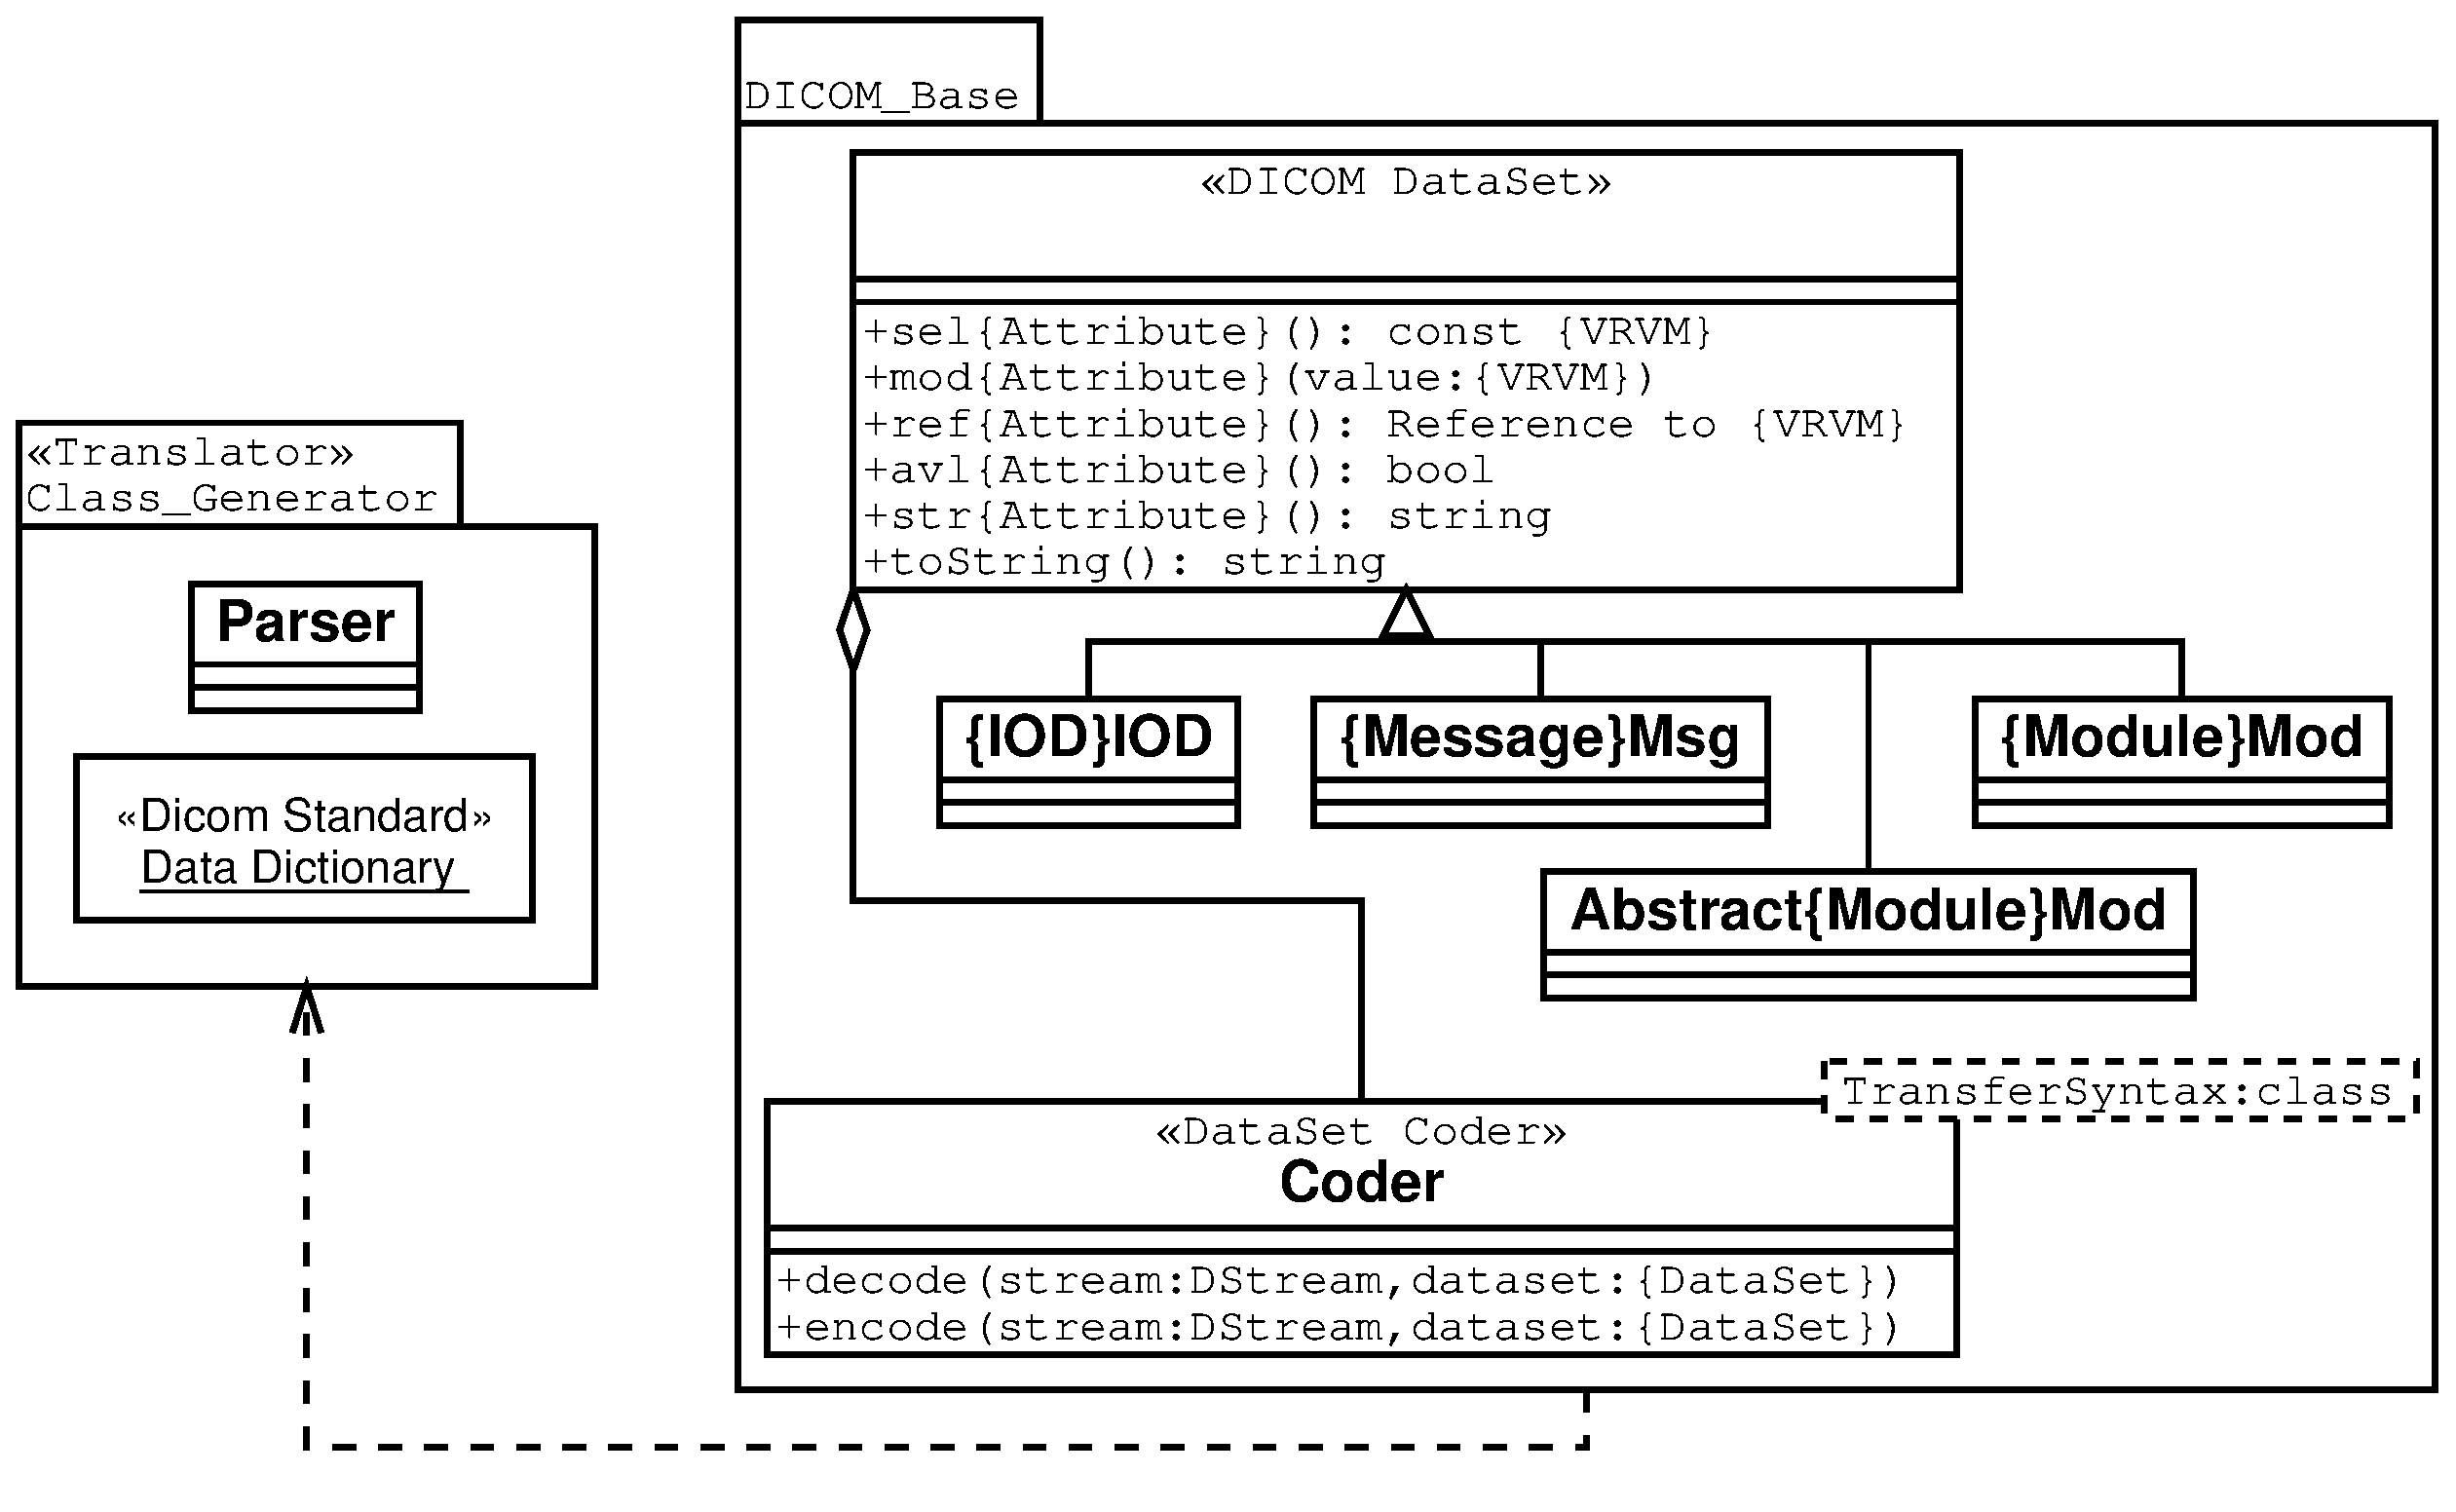
\includegraphics[scale=0.3]{medic-classgen.eps}
    \caption{A class generator translates DICOM Data Dictionaries into
      C++ code which becomes DICOM Base library.}
    \label{fig:classgen}
  \end{center}
\end{figure}

The major use of this approach was that the system was flexible, efficient,
understandable and reliable. The system proved to be flexible because adding
or removing a class or attribute was no burden. One could augment the class
system as quick as he could read it. Efficiency comes from the ability to
make use of built-in static C++ mechanisms such as inheritance instead of
implementing a custom one. The system was comprehensible because the adapted
classes were, in the interface, no worse than a typical C++ class; the DICOM
information model was translated at exactly the same level that it was
intended. Surely, reliability is a result of moving some operations like
type checking to compile-time; then, one can be sure that he is accessing
the right data type. Adapted classes, combined with a persistence mechanism,
is suitable for implementing DICOM SOP classes.


The output C++ code has classes named after information modules and IOD's.
A top level class contains attributes (with their types denoting their Value
Representation and Value Multiplicity, see PS3.5), selector and modifier
methods, string representation methods, and availability checking methods
for each attribute, nested Coder classes with all Transfer Syntaxes
supported. An IOD inherits from abstract super classes of its modules. The
IODs do not just aggregate the attributes from their modules, but inherit
their abstract interfaces. Also, sub-level classes were generated to be able
to implement the nested sequences (described in PS3.5). In addition to this,
the compiler handles mutually exclusive modules and DICOM pointer types. We
have made use of genericity features of C++, as well. The template mechanism
enables better setting of some of the key abstractions. We would like to
explain some of the abstractions at this stage. ``VR'' denotes a Value
Representation name such as US or AT in the following definitions.


\verb+Coder<class TS>+ classes These classes are responsible for the
encoding of an adapted DICOM class with a transfer syntax denoted by
TS. They are embedded within the class which they encode.

\verb+VR+ Value Representation with Value Multiplicity 1

\verb+VRf<int arity>+ Value Representation with a fixed Value Multiplicity of {`}arity{'} (ex. 3)

\verb+VRr<int lower, int upper>+ Value Representation with a Value
Multiplicity in the range lower-upper; i.e  1-10.

\verb+VRv+ Value Representation with a variable Value Multiplicity (1-N)

\verb+VRe+ Value Representation with an even variable Value Multiplicity (1-2N)

\verb+Seq<class SQ>+ Nested Sequence of sub-class SQ

The generated classes make use of standard C++ library for ease of use and
efficiency. Specifically, the boolean vectors Coders use are template
specialization vector<bool> classes.

Note that these classes are not declared within the generated code, but in
the other modules. The generated code is only a client of these classes. The
C++ programs are then compiled into a library module called MEDIC Base.

\subsection{Kernel}

For all these things to be operational, the complementary software should be
written and the required module is named MEDIC Kernel. The Kernel module
has two components:
Kernel low level and high level, with
the former defining the semantics required to compile auto generated classes
and the latter the whole interface.


% class environment
\newenvironment{class}[1]
{\textit{Class} #1:}
{
  
}
% end class env

\subsubsection{Low Level}

Kernel Low Level defines the following important classes as
well as those defined in the previous section.

\begin{class}{Tag}
  A 4 bytes tag which is unique for each attribute (see PS3.5). Also
  attributes are ordered by increasing tag number within a dataset when
  encoded.
\end{class}

\begin{class}{DPtr}
A pointer with a dynamic type that refers to an SOP instance. The DPtr
can check the virtual memory system to see if the instance really exists and
dereference.
\end{class}

\begin{class}{TransferSyntax}
  Base class for transfer syntax classes. The transfer syntax
  classes are static classes which supply low-level methods for data encoding
  and decoding. Each transfer syntax class handles these tasks differently.
  Currently, Implicit VR Little Endian, Explicit VR Little Endian, Explicit VR
  Big Endian transfer syntaxes are in use. It would be no matter to augment
  the remaining Transfer Syntaxes. Figure \ref{fig:transfersyntax}
  shows the present transfer syntax class hiearchy.
\end{class}

\begin{figure}[htbp]
  \begin{center}
    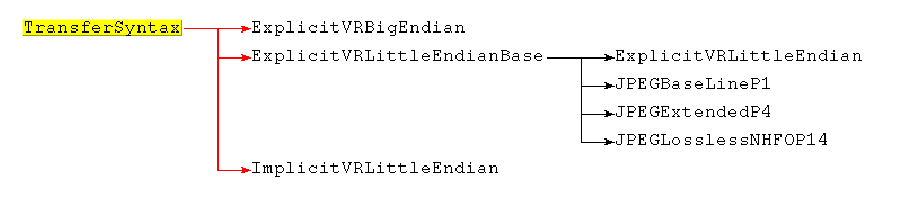
\includegraphics[scale=0.85]{transfersyntax-classhierarchy.eps}
    \caption{Transfer Syntax Class Hierarchy}
    \label{fig:transfersyntax}
  \end{center}
\end{figure}

\begin{class}{DStream}
  Base class for DICOM Streams. Descendants of this class manage
  streaming over TCP/IP and disk files. In figure \ref{fig:dstream},
  we see various descendants of DStream.
\end{class}

\begin{figure}[htbp]
  \begin{center}
    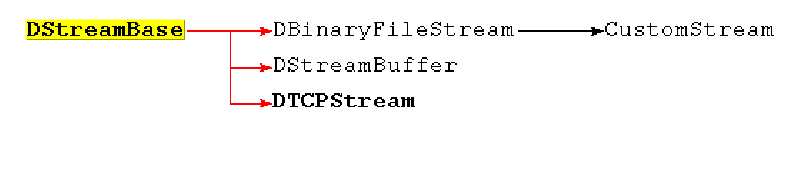
\includegraphics[scale=1]{dstream-classhierarchy.eps}
    \caption{DStream Class Hierarchy}
    \label{fig:dstream}
  \end{center}
\end{figure}

\subsubsection{High Level}

The high level portion of Kernel interface features:

\begin{class}{SOP}
  Abstract base class of all SOP Classes, this abstract class defines the
  minimal interface an SOP should support such as construction, destruction
  and encoding/decoding.
\end{class}

\begin{class}{DException}
  Base class for all DICOM Exceptions. Exceptions are thrown by
  many mechanisms in the system, for instance when a protocol error occurs.
  The DException has many subclasses which indicate different kinds of errors.
  The MEDIC user can catch and assess these errors.
\end{class}

\begin{figure}[htbp]
  \begin{center}
    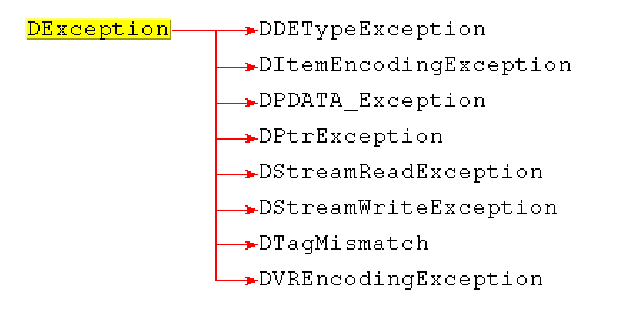
\includegraphics[scale=1.0]{exception-classhierarchy.eps}
    \caption{Exception Class Hierarchy}
    \label{fig:exception}
  \end{center}
\end{figure}


\begin{class}{DStreamBuffer}
  A stream buffer which implements DStream interface. This
  buffer is appropriate for PDU/PDV style input/output.
\end{class}

\begin{class}{DBinaryFileStream}
  A subclass of DStream which reads and writes to regular
  files.
\end{class}

\begin{class}{DTCPStream}
  A subclass of DStream which handles client stream connections
  over TCP.
\end{class}

\begin{class}{DServerStream}
  A special subclass of DTCPStream which is better suited for
  server connections.
\end{class}

\begin{class}{DApplication}
  This is the abstraction of a DICOM Application Entity. It is
  responsible for managing various configuration parameters and maintaining
  system data. There is only one instance of DApplication called dicom{\_}app
  in an application program.
\end{class}

\begin{class}{StorageManager}
  A class which implements a simple minded virtual memory
  scheme for large objects.
\end{class}

\begin{class}{DContext}
  The abstraction for a DICOM association, a subclass of DContext
  which manages execution of DICOM services.
\end{class}

\begin{class}{DTCPContext}
  Subclass of DContext which supervises both client and server
  association, and handling of DIMSE-C and DIMSE-N services within that
  association.
\end{class}

\begin{class}{DFileContext}
  Subclass of DContext responsible for reading and writing DICOM
  files. This class implements a tentative subset of DICOM File Services
\end{class}

\begin{class}{DImageStacker}
  This class is declared if MEDIC{\_}ARCHIVE symbol is defined.
  The class checks to see if a series is complete and if so sends a special
  message to the archive system.
\end{class}

Within the MEDIC Kernel, platform specific features are kept minimum and ANSI
C++ library is used for all elementary data structures:
\verb+list<T>+, \verb+vector<T>+, \verb+map<K,T>+ are used extensively.

\subsection{Platform}

This part of MEDIC is platform specific. The following classes employ
the platform specific services to obtain  desired functionality. On
WIN32 platforms, MFC is used to that end and on POSIX we use pthreads
and BSD socket library.

\begin{class}{ListenerSocket}
  Subclass of Socket that listens to the DICOM port of AE
  all the time spawning children server connections appropriately.
\end{class}

\begin{class}{ListenerThread}
  dicom{\_}app started thread which initiates the DICOM SCP.
\end{class}

\begin{class}{CustomSocket}
  Subclass of Socket which is capable of processing PDUs.
\end{class}

\begin{class}{ClientSocket}
  Subclass of CustomSocket which is intended for client
  connections, sends a message to calling thread on end of transmission.
\end{class}

\begin{class}{ClientThread}
  Thread that is started when a client connection is going
  underway.
\end{class}

\begin{class}{ServerSocket}
  Subclass of CustomSocket which is intended for server
  connections. On receipt of a PDU it executes its DTCPContext which is in
  server mode.
\end{class}

\begin{class}{ServerThread}
  Thread that is started when a new server connection is made.
\end{class}

\begin{class}{CTEmulator}
  A dialog which essentially emulates a CT machine that can perform
  various DICOM operations for testing.
\end{class}

\section{Policies}

\subsection{User Protocol}

The application programmer adheres to some conventions to assure DICOM
compliance. The user is committed to the deployment of SCU only, the SCP is
handled automatically by the DCL system.

Client programming is straightforward, since the DCL does not support
asynchronous operation. Calls to DICOM services do not return until
completion or error occurrence. Generally, the user works on the SOP
instances, and applies DICOM services over Context classes. Currently, two
Context classes are supported, first of which is DTCPContext and second is
DFileContext.

With DTCPContext, the user first establishes an association with a SCP
Application Entity; then, the programmer performs any number of DICOM
services with the peer AE\@. Fatal errors cause exceptions to be thrown; it is
advisable that the programmer handles exceptions. After all operations
cease, the MEDIC user closes the connection by releasing the association. On
the other hand, with the DFileContext, the user can read and write single
DICOM files. Note that the DICOM directory structure is not yet implemented.

\subsection{Build System}

We use two different build systems for two main families of operating
systems. On POSIX platforms, we use automake/autoconf and on WIN32 we
use Visual C++'s integrated build system. Build settings for both
kinds of platforms are provided in the distribution.

\subsection{Source Code Organization}

\subsection{Notes to Developer}

One should contemplate the structure of MEDIC in eloquent fashion when he
wishes to improve it. The following sections depict a developer's account
of the library.

\subsubsection{Sketch Board}

The MEDIC is the result of our vision of a robust system that employs DICOM,
therefore the library has not been pictured as a black box which supports
some of the standard but rather as an animate company to it. The
architecture naturally exposes some deficiencies, however it is our belief
that they can be remedied with little labor. The developer must reckon that
the object-oriented design should be maintained, with the class semantics
closely paralleling that of concepts in the standard. Whenever the rational
connections dissolve into daily fixes, the library must be revised. We have
considered that the primary issue is to facilitate the making of DICOM
compliant application programs: the conformance of the library is not
sufficient by itself. Then, the features that an application programmer
anticipates should be in the library. One implication of this statement is a
rule of minimal usage, the application programmer expects to give only the
required information to a subsystem, that is he wishes to confront a slim
interface, with the chance of selecting beyond default modes of operation.

As seen in some example code fragments in the DICOM documents, a programmer
wants to open an association, command some DICOM messages sequentially , and
shut it down; besides there is a high contingency that he would like to
direct the objects in a smooth fashion. We concede then, that the programmer
must be able to perform all these tasks simply and efficiently. The MEDIC is
adjusted towards making common operations easier while allowing fancier
ones. We have first concentrated on the object system, inheritance
relations, abstract classes and methods, information retrieval and
manipulation, then moved on to decoding/encoding, message passing and
application framework, always taking these aspects of design into account.

\subsubsection{How to Start a MEDIC Application}

There is an example in the source tree which demonstrates how to use the MEDIC
for implementing a DICOM Application Entity. The project is called
CTEmu. This is an example code that does some of the DICOM operations a CT
machine might perform.


\subsubsection{Configuration Files}


MEDIC, by default, checks some configuration files in the directory it is run
in. The distribution directory must therefore populate some tiny text files
within the ./etc directory to successfully open the library

ae-config.txt: file contains three words, name of the application entity to
run (not to exceed 16 characters, conforming to AE primitive data type),
DICOM TCP/IP port, and a numerical identifier for the application entity
(used in UID generation)

dicom-Aes.txt: file contains an entry for each known Application Entity.
Each entry consists of three words: name of the AE, TCP/IP address, and
DICOM port number respectively.

storage.txt: file holds two words: maximum number of megabytes to use for
local disk storage, and maximum number of megabytes the application program
can occupy in memory. These values directly affect the custom virtual memory
mechanisms in MEDIC.

Example of these files may be found in the ./dist directory in the main
source tree.


\subsubsection{SOP Architecture}

One vital point for the library client and developer is the structure of
SOP{'}s in the MEDIC. As previously stated, MEDIC makes use of compile-time
classes for the several IOD{'}s, Modules and Messages in the standard; that
is they are conventional C++ classes. However an SOP is not merely composed
of a data structure, but pertains to a set of client services which
incorporate DICOM messaging. Assuredly, SOP is a fundamental abstraction in
the whole library.



MEDIC SOP{'}s have a fairly simple minded organization. A class called SOPs
registers all known SOP classes, the SOPs class has an instance within the
DApplication, so features a single instance in the application. SOPs is also
a proper place to do class-wise initializations except registration for the
SOP classes.



The SOP interface is explained in the MEDIC Reference section, however some
elaboration is required. First of all, the SOP addresses some raw
functionality and expects a higher level construct to make use of them (such
as decoding/encoding). The actual category of such classes are DContext
descendants. Furthermore, since composite SOP classes and normalized SOP
classes represent a high level of genericity, they are handled by template
classes. One template class is defined at present: the
CompositeSOPClass<class IOD>, though a NormalizedSOPClass<\unskip\ldots> is
also required. The difference emanates from the fact that the normalized SOP
classes do not always have class and instance ID{'}s in the SOPCommon
Module.



\subsubsection{Adjoining an SOP Class}

The library purposes to support all DICOM Composite SOP classes, so addition
or removal of a class should be made effortless. The addition of an SOP
Class is realized in a few simple steps. First the programmer checks whether
the data structures have been generated. If the required module and IOD
definitions are absent, the programmer revises the relevant dictionaries,
and generates the C++ classes which go into the ./dcl-gen directory. Then,
the MEDIC Base Library configuration is altered so that the necessary modules
and the IOD are compiled in. Succeeding that, a declaration similar to


\verb+typedef CompositeSOPClass<CTImageIOD> CTImageStorage;+


is appended to the SOPClasses.hxx interface file. Then the static members of
the SOP Class must be defined, probably in SOP.cxx file. In addition to
this, the initialization method of SOPs class must be altered so that the
new SOP Class gets registered. It might be a good idea to automate some of
this process by expanding the class generator, so that for instance the
registration routines are also automatically generated.


\subsubsection{Getting C-GET Done}

DICOM C-FIND and C-GET services demand a lot of attention whilst
implementation. These services are in fact simple query services, with the
C-FIND reporting what instances have been found, and C-GET returning
instances themselves. However, there is more to the discussion. Firstly, the
query services have a slightly alternate decoding/encoding for the
indication of keys to command the query, this combined with the wildcard and
range matching specifications make a significant burden. Secondly, and more
important than the previous issue, the information model must suit the
C-FIND/C-GET query model. The minimum implementation of the query services
demand a patient rooted hierarchical information model with a wide choice of
keys from each level of the hierarchy. The database developed for our PACS
system, indeed has a hierarchical model as required, but plenty of the keys
are missing.



The clever thing to do is to think in terms of client and server. The client
part needs a way to indicate any kind of query that can be made. This could
be over a special dataset, which goes into the query definition of the
request message. Also, the client must collect the response is composed of
multiple response messages into a simple structure and present them to the
application programmer. The server side is more elaborate, however, it seems
as though a single SQL statement construction is possible. As the keys are
interpreted, one by one, the single statement could be grown iteratively to
match the query. When, as the result of the query, instance UID{'}s of the
requested SOP instances are retrieved from the database, they can be cast
into the response. According to the type of service (the query service
C-FIND, or the retrieval service C-GET) ID{'}s or instances themselves are
emitted. The bottleneck here is the interpretation and forming of the SQL
statement. Quite elaborate handling of the query types and codings is
required, also the database must be tuned to fit the queries


\subsubsection{Graceful DICOM Association}

All DICOM application entities must implement the DICOM Protocol Machine.
The machine is convoluted in nature, and works by passing by PDU{'}s
according to a FSM. The establishment and closing of the association is very
important and must be tested severely, since all DICOM operations depend on
a live association. The protocol machine in MEDIC has been implemented in an
elegant fashion, however it has incomplete parts. For a graceful association
every possible move of the protocol machine must be handled and caressed.
Effectively, the ARTIM timers and presentation context passing is missing in
the MEDIC protocol machine. However, since the infrastructure is complete,
little work remains. In the case of ARTIM timers, in some events a timer
must be started, and the time-out causes the connection to close. The timers
were not required for the test purposes, so they were omitted. However
implementing the timers is not tricky. A single NT timer should be allocated
at all times, with the other timers handled via timer queue. (NT has a
limited number of timers) For presentation context implementation, only the
associate client and server methods in the DTCPContext have to be dealt
with. The associated PDU{'}s are in majority complete, and plugging in a
presentation context in the DTCPContext class must not be much of a problem.
On that occasion, the PDV list passing must also be completed to full
operation and efficiency.

Another advise would be separation of DTCPContext into a client class and a
server class. Moreover, clustering DICOM Service Groups into corresponding
classes is a good idea. Print Management has been done in that fashion.

\subsubsection{Delicate Points}

Unfortunately, the library is not at the point of perfection, so future
tasks have to be enlisted. The fleeting descriptions may not be exhaustive,
nevertheless they elucidate the crucial issues.

Modulewise operations which work at the level of an information module are
required. By these operations, one should be able to tell existence of a
module (so that the application programmer may interpret which role an
object has taken), copy, extract or move a module with the module classes.
The mutually exclusive parts of some IOD{'}s should also be considered at
this stage. The MUTEX keyword in the class generator is handled rather
awkwardly, that should be refined also. The handling of mutually exclusive
parts would make the system superlative.

Handling pointer identifiers better in IOD::add{\_}module() is suggested.
Although no conflicts arise, pointer identifiers should be checked for
collisions.

50xx and 60xx Repeating Groups are discarded altogether, for they stand as
ad hoc mechanisms in the standard. Developer should Decode/Encode Repeating
Groups appropriately, probably by putting in a flag in auto-gen Attributes
and handling of repeating groups in Transfer Syntaxes. As the standard
suggests, repeating groups are to be replaced by ordinary sequences, so the
wisest solution is to represent repeating group modules as sequences, then
while decoding/encoding perform suitable conversions.

Conditional Requirement Types are omitted currently, those types are coerced
into optional ones. Of course that should be corrected by making an
extensive condition mechanism. The most common condition is the existential,
so that must not make much of a hardship for the classgen.

For the time being, first attribute of each module is scanned, and if they
are not there, a skip flag for that module is set, which makes decoders of
that attribute optional. Collisions do not have to be handled separately
with this scheme.

The compile-time coders are a good idea, however it has little flexibility.
The current scheme disregards error recovery while parsing. On any error,
including even the slightest of protocol violations, the system comes to a
halt and throws an exception. The solution comes from enriching the
metaclass information within dataset classes. In the auto generated classes,
there is attribute information, adequate to some extent: one can dump an
attribute{'}s properties. Still and all, the information is not tied in. The
ingenious course is to write a decoder/coder method for each attribute and
relate them with static member pointers for each attribute which are,
surely, contained in a static data structure of the coder class which are in
parallel with the attribute container in the dataset class. Thereupon, the
library developer may translate some of the compile-time mechanisms to
run-time, getting a bit more freedom of action. The resulting coder is a
ephemeral algorithm which iteratively parses each attribute (in the encoding
order) from the data structures just mentioned, and handles some of the
exceptions appropriately, cushioning the application programmer from
frequent DICOM disasters.

On careful inspection of library internals, one is likely to find some flaws
with the streaming technique. There are unfortunately two methods for
streaming, one depends on some internal private routines in MFC extension,
and the other uses custom stream buffers. The stream buffer approach is more
elegant, and the former must be replaced by it. Meantime, it would be
incredibly useful to draw a base class for stream buffers and derive
specializes input and output stream classes. Despite the peaceful execution
of stream routines, these measures should be taken.

\section{Detailed System Design}

Detailed System Design consists of a class reference manual which
is in a separate document.

\end{document}
